%-----------------------------------------------%

% PREAMBLE %

%-----------------------------------------------%
\documentclass[a4paper,12pt]{article}

% Packages
\usepackage{graphicx}
\usepackage{amsmath}
\usepackage{geometry}
\usepackage{fancyhdr}
\usepackage{setspace}
\usepackage{titlesec}  % For title formatting
\usepackage{tocloft}
\usepackage{xcolor}
\usepackage{enumitem}


% Header and Footer
\pagestyle{fancy}
\fancyhf{}
\fancyhead[L]{Abereni Opuiyo}
\fancyhead[C]{PHY121}
\fancyhead[R]{\thepage}
\fancyfoot[L]{Lab Report 4: Free Fall}
\fancyfoot[R]{\thepage}
\geometry{margin=1.2in}
\setstretch{1.5}
\renewcommand{\footrulewidth}{0.1pt}% default is 0pt

% Table of Contents
\renewcommand{\contentsname}{Table of Contents}
\renewcommand{\cftsecleader}{\cftdotfill{\cftdotsep}}



% Title Formatting
\titleformat{\section}{\normalfont\Large\bfseries}{\thesection}{1em}{}


% Cover Page
\title{
    \vspace{5cm} % Adjust vertical space
    
\includegraphics[width=0.55\textwidth]{dutchess-logo-blue.png} \\ % Add your logo here (change "logo.png" to the actual filename)
    \vspace{1cm} % Adjust vertical space after the logo
    \textbf{\Huge Lab Report 4: Free Fall} \\
    \vspace{1cm} % Adjust vertical space
    \large PHY121 \\
    \vspace{0.5cm} % Adjust vertical space
    \large	October, 3rd, 2024 \\ 
		\vspace{.5cm}
		\large Professor R. Lathrop | Professor T. Zito
}
\author{Abereni Opuiyo}
\date{}
%-----------------------------------------------%

% TITLE PAGE %

%-----------------------------------------------%
\begin{document}
\maketitle
	\thispagestyle{plain}
\newpage

%-----------------------------------------------%

% Table of Contents  %

%-----------------------------------------------%
% Start page numbering from the Table of Contents

\setcounter{secnumdepth}{0}
\setcounter{page}{1}  % Start counting from 1
\tableofcontents
\thispagestyle{fancy}
\newpage

%-----------------------------------------------%

% Purpose  %

%-----------------------------------------------%

\section{Purpose}
\vspace{-0.5cm}
\singlespacing
The purpose of this lab was to measure the acceleration due to gravity by dropping an object through a timer and recording its motion.Using the data we collected, we determined the approximate rate at which the object's velocity changed in the air.

%-----------------------------------------------%

% Theory  %

%-----------------------------------------------%

\section{Theory}
\vspace{-0.5cm}
\singlespacing

\indent If \textit{velocity} is the rate \& direction of an object's \textit{position} over a certain time interval, then \textit{acceleration} is the rate \& direction of an object's \textit{velocity} over a certain time interval. So long as an object's velocity is changing, it has acceleration.\par 


Velocity and acceleration are both \textit{vector} quantities, meaning both have vertical and horizontal components. The vertical component of an object's acceleration is impacted by the Earth's gravity. The acceleration due to gravity on Earth's surface has been measured to be \textit{$9.80 {m/s^2}$}. \par

\begin{figure}[h!]
    \centering
    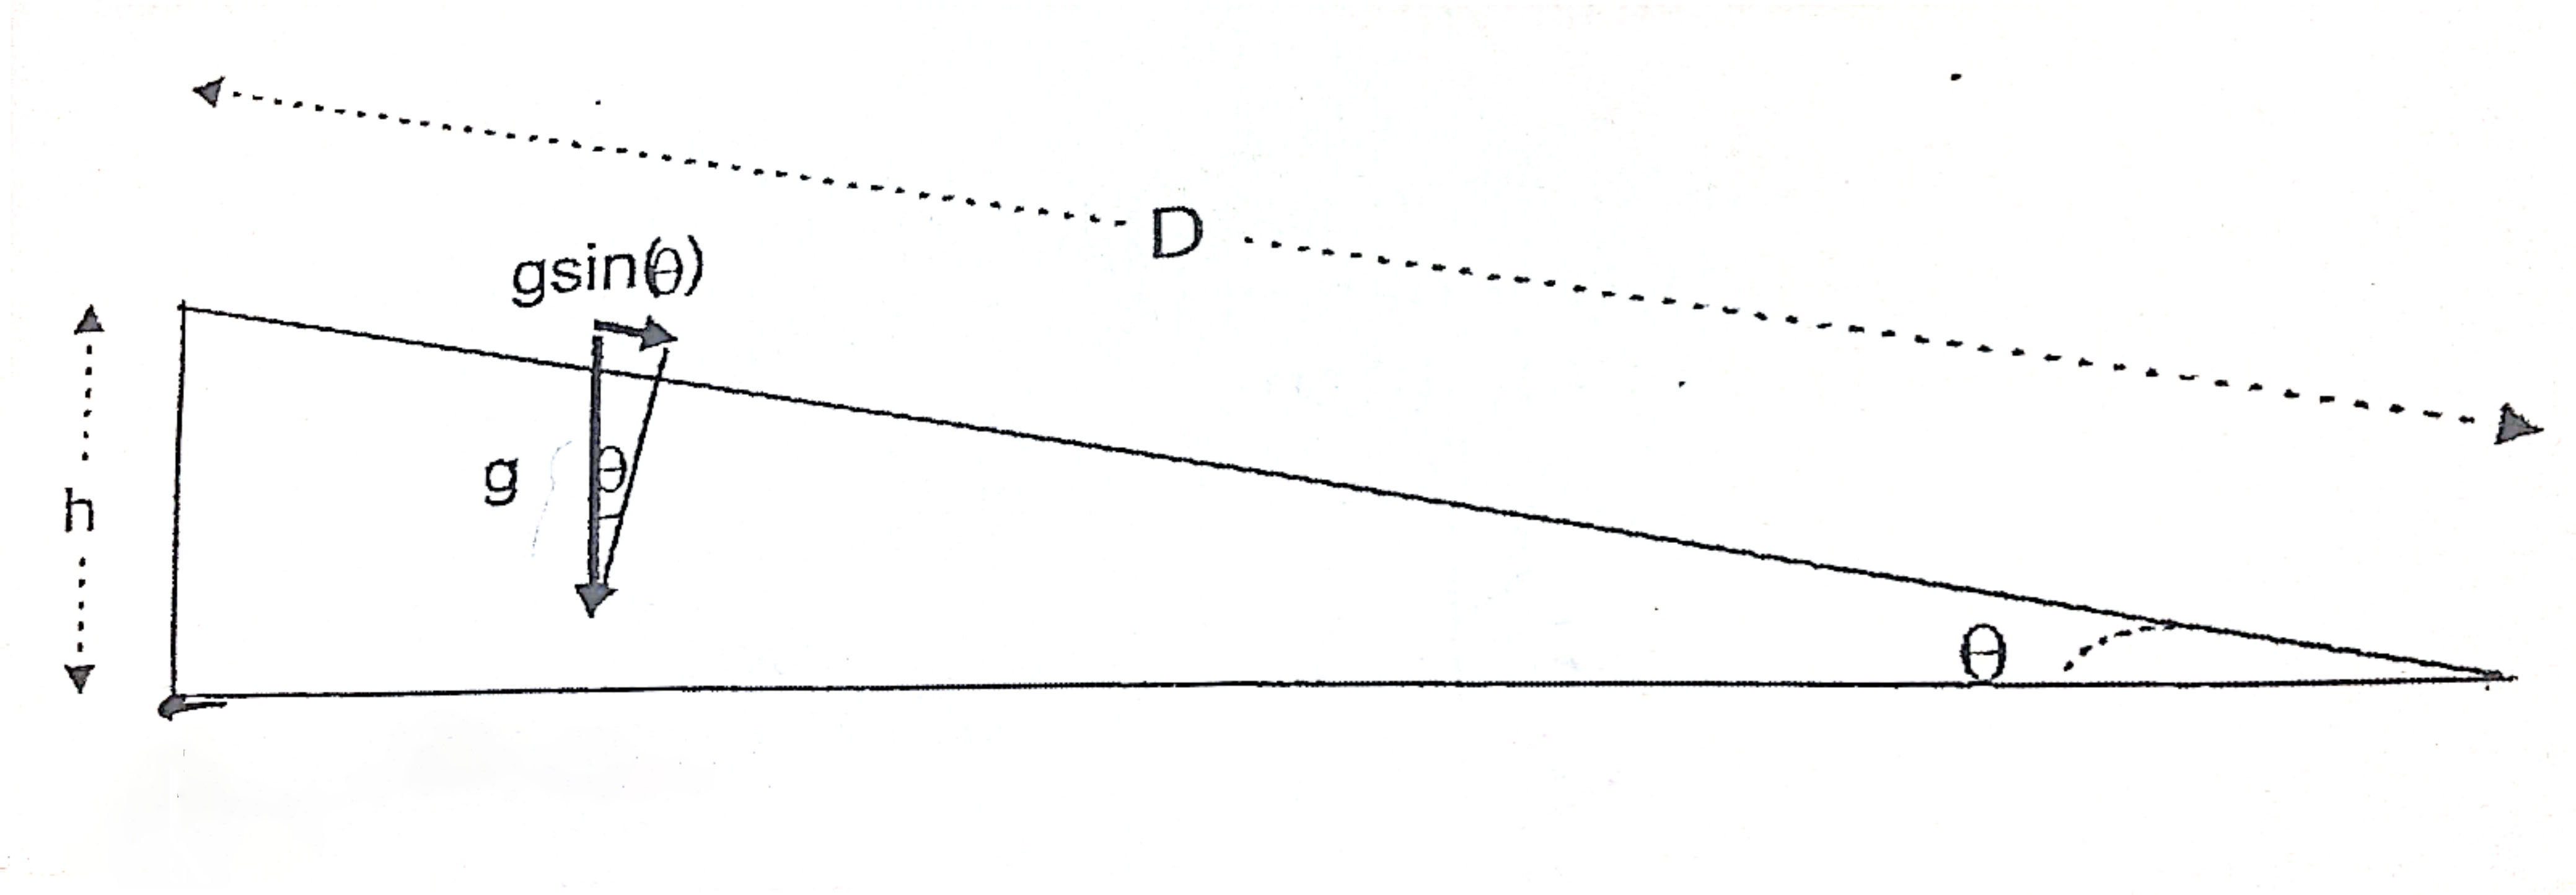
\includegraphics[width=0.8\textwidth]{figure1_inclineplane} % Example of adding a figure
    \caption{Incline plane}
    \label{fig:inclineplane}
\end{figure}

When objects fall straight down, assuming there's no air resistance, the vertical component of the object's acceleration is simply $9.80 {m/s^2}$. However, if the object is launched at an angle, then the object's acceleration in the vertical direction must be determined in a different way. Just as one would determine the horizontal \& vertical components of velocity for objects thrown at angles using trigonometric functions, so too can the acceleration due to gravity of such objects be calculated. More specifically, for objects that move along \textit{inclined planes} (see figure \ref{fig:inclineplane}), the component of the acceleration vector parallel to the plane can be calculated with the following equation:

\begin{equation}
a = gsin\theta
\label{eq:1}
\end{equation}

The plane angle (figure \ref{fig:inclineplane}) can be determined using:

\begin{equation}	
sin\theta = \frac{\Delta{h}}{D}
\label{eq:2}
\end{equation}

\newpage


%-----------------------------------------------%

% Procedure  %

%-----------------------------------------------%


\section{Procedure}
\vspace{-0.5cm}
\singlespacing


%Free Fall

\subsection{Free Fall}

\subsubsection{Setup}

	\begin{enumerate}

		\item Plugged in \textbf{Accessory Photogate Timer} into Ch. 1 on \textbf{Lab Pro} interface
		\item Opened \textbf{Logger Pro}
			
		\item Tested sensor by pressing \textit{"collect"} on \textbf{Logger Pro}
	\end{enumerate}	

\subsubsection{Measure Times \& Find Acceleration}
	\begin{enumerate}[resume]

		\item Dropped \textbf{picket fence} vertically
	
		\item Recorded data from \textit{Velocity vs Time} plot

		\item Calculated slope of velocity by hand and record your calculations

		\item Used the linear regression function on \textbf{Logger Pro} to find the average velocity of the object

		\item Saved graph of acceleration

		\item Repeated steps 4-5, 5 more times and recorded the average acceleration of the trials
	\end{enumerate}

\subsection{Inclined Plane}

\subsubsection{Setup}

	\begin{enumerate}
		\item Connected \textbf{Motion Detector} to \textbf{Lab Pro} 
		\item Tested sensor by pressing \textit{"collect"} on \textbf{Logger Pro}
		\item Placed sensor at bottom of track
		\item Used a \textbf{meter stick} to measure 0.4m of distance between the motion sensor and the cart and marked it.
	\end{enumerate}

\subsubsection{Starting at the Top}

	\begin{enumerate}[resume]

	\item Held cart at marked spot and released it
	\item Recorded average acceleration of linear region in the data using linear fit function in \textbf{Logger Pro}
	\item Repeated steps 5-6 another 3 times 
	\item Calculated and recorded average acceleration of cart during the 4 trials
	\item Used \textbf{meter stick} to measure D and h of the track as described in figure \ref{fig:inclineplane} to calculate angle of track using equation \eqref{eq:2}
	\item Calculated difference between average acceleration in trials and acceleration from equation \eqref{eq:2}
	\end{enumerate}

	\subsubsection{Starting at the Bottom}

	\begin{enumerate}[resume]
			\item Practiced pushing cart up track at least 0.4m from the motion sensor
			\item Recorded motion of track when moving from the bottom and calculated its acceleration.
			\item Repeated and recorded motion trial 3 more times, then calculated average acceleration
		\end{enumerate}


%-----------------------------------------------%

		% Calculations & Graph   %

%-----------------------------------------------%


\section{Calculations \& Graphs}

\vspace{-0.5cm}
\singlespacing
%-----------------------------------------------%

% Questions  %

%-----------------------------------------------%


 \section{Questions}

\vspace{-0.5cm}
\singlespacing

\begin{enumerate}
	\item \textbf{What do you expect the acceleration of the picket fence to be?Is it exactly this value? If yours is higher or lower provide explanations as to why that might be.}

		We expected the acceleration of the picket fence to be around $9.8 {m/s^2}$. Our calculations ended up being slightly slower but well within 10\% of difference. The difference in values could be due to air resistance, or the small breeze produced by multiple bodies moving at the same time in a room.

	\item \textbf{Do you expect that the detector's measurement of time is exactly correct? What might afect the detector's measurement of time?}

	It's very possible that the detector has a few milliseconds of delay so the measurement of time wouldn't be completely accurate. It's alsopossible that the detection algorithm of the device is finely tuned such that the minute blending of colors at the borders on the picket fence would also cause times to be off.

	\item \textbf{What is your average value, standard deviation, and relative error for the acceleration due to gravity, g?}

	
\end{enumerate}


%-----------------------------------------------%

		% Conclusion %

%-----------------------------------------------%


\section{Conclusion}

\vspace{-0.5cm}
\singlespacing

\end{document}



